\documentclass[11pt]{article}
\usepackage[margin=1.2in]{geometry}
\usepackage{graphicx}
\usepackage{fancyhdr}
\usepackage{nopageno}%removes number on titlepage
\usepackage[parfill]{parskip}
\usepackage{subfig}
\usepackage{multirow}


\begin{document}
% Cover page
\author{Chelsey Legacy, Lindong Zhou, Evan Pete Walsh\footnote{Statistics graduate students at Iowa State University of Science and Technology}}
\title{STAT 579 Final Project}
\maketitle

\begin{abstract}
Analysis of the Yelp Academic Dataset.
\end{abstract}

\newpage

\tableofcontents

\newpage

\pagenumbering{arabic}%starts numbering at "1"
\pagestyle{fancy}
\fancyhead[L]{Iowa State University}
\rhead{\thepage}
\rfoot{\today}
\cfoot{}%removes default page number at bottom center


\section{Introduction}

Lindong


\section{Data}

The Yelp Academic Dataset\footnote{$https://www.yelp.com/academic\_dataset$} provides data enthusiants with the exciting opportunity to explore an incredible collection of information regarding the characteristics and quality of hundreds of businesses across the United States, Canada, and the UK. Specifically, the data includes details and reviews on 250 of the closest businesses to 30 large universities, including the Arizona State, UNLV, the University of Edinburgh, the University of Wisconsin, and the University of Waterloo, to name a few. The raw data is in json format and contains five different types of json objects: \textbf{Business}, \textbf{Review}, \textbf{User}, \textbf{Check-in}, and \textbf{Tip}.

Each \textbf{Review} object represents an individual user-based review of a particular business. The unique encrypted business ID is given along with the date of the review, the number of stars (out of 5) that were awarded, the number and type of votes that the review received, and an optional text description provided by the user. \textbf{User} objects are unique to every person that has an active Yelp account. Each user has a name, a unique encrypted user ID, the number of votes they have cast, the average number of stars they have given, and the date they signed up for Yelp, among other things. A \textbf{Check-in} object represents the count and time of all the registered check-ins for a particular business, and \textbf{Tip} objects represent a tip given by user for a particular business. Tips include the user's ID, the business's ID, the date, and the message that the user gave. While these objects all provide a rich source of information, for the scope of this paper we will only be examing the \textbf{Business} objects.

\textbf{Business} objects are unique to business ID's, and include the following information:
\begin{itemize}
	\item the name of the business,
	\item the name of neighborhood in which the business is located,
	\item the city in which the business is located,
	\item the full address of the business,
	\item the exact latidude and longitude coordinates of the business,
	\item the average number of stars awarded to the business,
	\item the number of reviews received by the business,
	\item whether or not the business is still open,
	\item the hours that the business is open,
	\item the categories that the business falls under,
	\item and a number of different attributes which mostly concern restaurants and bars, such as whether or not smoking is allowed and the price range of the food.
\end{itemize}

To work with the data, we converted the set of all \textbf{Business} objects to a csv file in which the columns are variable names representing each aspect of a \textbf{Business} object, and each row corresponds to a unique business. Each different type of attribute was converted to its own character, numerical, or logical variable depending on what was appropriate. For example, the attribute \textbf{smoking} was converted to a logical variable where the value is ``true" if the smoking is allowed at the establishment, and ``false" if it is not allowed, while the attribute \textbf{price range} was converted to a numerical variable which ranges from 1 to 4.

\section{Restaurants}

\subsection{Breakfast}

\subsection{Lunch}

\subsection{Dinner}

\subsection{Food By Type}

\begin{figure}[h!]
  \caption{Plot of the counts of each type of food filled by if they have delivery or not.}
  \centering
  \label{delivery}
    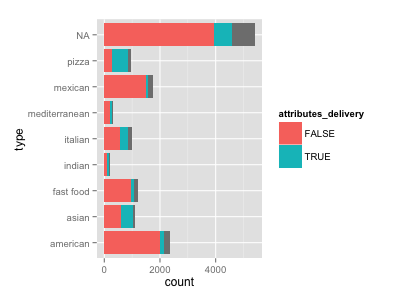
\includegraphics[width=0.5\textwidth]{Figures/delivery.png}
\end{figure}

In a world where people lead busy life styles and have little time to cook, sometimes we may be forced to call out for delivery.  But what types of food are most likely to have delivery?  In other words, if we are ordering out what is it likely we will be able to have delivered to us? In 
igure~\ref{delivery} we can see that the food types that most likely have delivery are those that serve pizza, asian, or possibly italian.  Most likely you will not be able to find an American or fast food place that delivers.  This could be due to the fact that some of these food do not stay good if they sit too long.  Food like pizza and rice are fine to sit for a while and are easy to keep warm and fresh tasting, and can also be easily reheated. Thus, these are qualities that make them good options for delivery.  However, american food, or fast food like burgers and fries are not good if they sit too long, and do not reheat to the quality they were when they left the restaurant.  
\section{Bars}

The Business dataset contains a lot of information that can be used to analyze the relationship between different aspects of bar culture.  In order to analyze the bars available in the dataset, the data was subset to get rid of any businesses that did not have a full bar.  Looking at only the businesses with a full bar gives us insight into locations that serve from a full bar such as clubs, hotels, select restaurants, lounges, bowling alleys, and other various entertainment locations.  Through analyzing this data we can explore what attributes are likely to get a bar higher rating, what features bars most commonly share, and if lower ratings indicate a bar   
could shut down.

\subsection{Food}

\begin{figure}[h!]
  \caption{Plot of the number of stars a restaurant received filled with the type of food served at the bar.}
  \centering
  \label{food}
    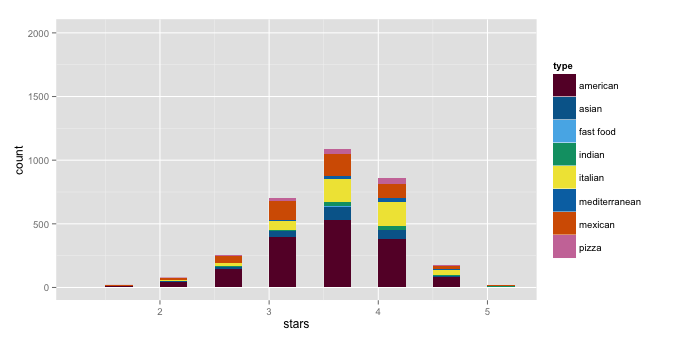
\includegraphics[width=0.5\textwidth]{Figures/Food_bars.png}
\end{figure}

Though not all bars serve food, many bars in restaurants do which begs the question; what is the most common food served in bars?  In order to investigate this question a qplot of the number of starts given to each bar filled with a count of the food types for each different rating will give us the information and more.  This data revealed unsurprisingly that the most common food served in American bars is American food (burgers, fries, etc). Through further analysis it is determined that 50$\%$ of the bars served primarily American style food.  We can see that the majority of each bar of star, no matter what the rating, is colored for American food.  However, looking more closely at the graph we can see that there is some unexpected information.  From Figure~\ref{food} we can see that there are a wide number of food options for people looking for full bars.  Along with American, Italian and Mexican are also abundant options making up 16$\%$ and 16.7$\%$ respectively.  Another piece of information we can infer from this graphic is that along with the plot of the stars a bar receives being a normal distribution, there also is a consistency in the number of each type of food being represented at each level of stars a bar receives.  Thus, we can see there is no preference for food when looking for a certain quality bar. A bar is equally likely to serve American food whether it receives 1 star or 5 stars.  This could be further investigated through hypothesis testing for difference in proportions.

\subsection{Stars}
\begin{figure}[h!]
  \caption{Plot of the number of stars a bar received colored by whether or not they are open or closed}
  \centering
  \label{open}
    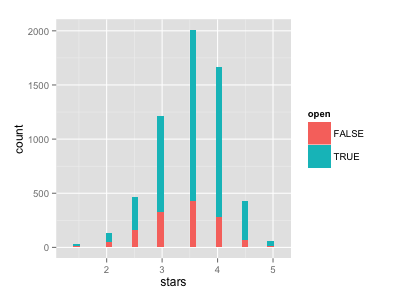
\includegraphics[width=0.5\textwidth]{Figures/barstatus.png}
\end{figure}
The purpose of yelp is to provide review of businesses for others in the community to take into consideration.  Since this dataset provides the number stars a bar receives and the status of the bar (open or closed) as of when the data was collected.  I decided to investigate the idea that possibly if the bar has lower ratings it has more of a chance of being closed.  It is hard to discern any sort of relationship from the plot, except that there are more restaurants open than closed.  However, if inspected closely looking at the extreme endpoints of the graph you can see it appears the percent of open restaurants at the 5 star level is higher than the percent of 1 star restaurants that are open. In order to look into this further I created several subsets of the data.  I created a subset of data for 2 stars(1 star had 0 observations), 3.5 stars (which is the median of the data), and 5 stars.  I then found the percent of open bars for each level.  I found that the 2 stars had 64.3$\%$ open, the 3.5 stars had 78.4$\%$ and 5 stars had 82.1$\%$ open.  As we can see the percentages of bars open increases as the number of stars the bar is rated increases.  Though we can make no assumptions of causation, this is still an interesting trend tp consider for further more complex analysis.

\subsection{Popular Features}

Each bar in a community has its own unique features, special pricing promotions, or atmosphere.  Some bars are good for dancing, watching televisions broadcasting sports games, happy hour, or some are more quiet and laid back for just talking and relaxing with friends.  What are the relationships between these variables, if any?  I wanted to find characteristics for each of the  different atmospheres a bar may have: romantic, intimate, touristy, hipster, divey, classy, trendy, upscale, and casual.  However, it quickly became clear that there are not many bars in each of these categories.  Most bars are just causal. 


\begin{figure}[h!]

                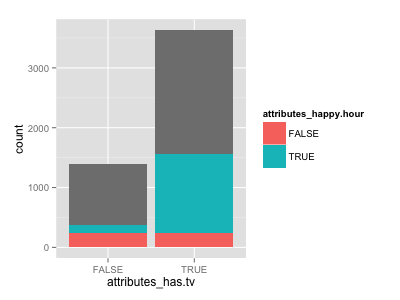
\includegraphics[width=0.5\textwidth]{Figures/tvhappyhour.png}
                \caption{Plot indicating whether or not the bar as a tv, colored by if it has happy hour specials.}
                \label{happy}
        \end{figure}
   
        \begin{figure}[h!]
                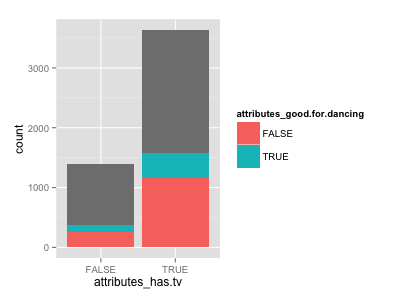
\includegraphics[width=0.5\textwidth]{Figures/tvdancing.png}
                \caption{Plot indicating whether or not the bar as a tv, colored by if it is good for dancing}
                \label{dance}
        \end{figure}
 


Next, I thought it would be interesting to look at features of bars with televisions.  Since, not all bars have televisions there must be certain characteristics for those that choose to have a television and those that do not.   In  Figure~\ref{happy} we can see that most bars that have a tv also have happy hour specials.  These are probably more causal places that people go after work to relax with coworkers and friends.  We can gain even more insight into the bars with tvs when we look at  Figure~\ref{dancing}.  In this plot it is interestingly apparent that if a bar has a tv it is more likely that it is not good for dancing.  This again reinforces that the bars with televisions are more of a relaxed atmosphere, or a sports bar.  Most likely a place like this would be an in inappropriate atmosphere for a group looking to go dancing.  Places people go dancing are more apt to be louder places people go later at night, when happy hour specials would be over and there would be no need for televisions.
                      





\section{Hotels}

Lindong

\section{Fitness}

Lindong


\section{Conclusion}


Chelsey




\end{document}